\documentclass{article}  % //TODO find why latex gives errors for report and using textsc!
\usepackage{fancyhdr}
\usepackage{graphicx}
\usepackage{amsmath}
\usepackage{mhchem}
\usepackage{amssymb}
\usepackage[margin=1in]{geometry}

\graphicspath{{./images/}}

\title{UW CHEM 152 Notes}
\author{Anthony Le}

\newtheorem{exmp}{Example}
\newtheorem{exrc}{Excersize}
\newtheorem{proof}{Statement}
\newtheorem{defn}{Definition}


\begin{document}

\pagestyle{fancy}
\fancyhead{}
\fancyhead[R]{UW CHEM 152}
\fancyhead[L]{Anthony Le}

\begin{center}
    \LARGE{\textbf{CHEM 152 ALEKs Scratch Work}}
\end{center}

Create ICE Table \\
\begin{tabular}{c|c@{}c@{}c@{}c@{}c@{}c@{}c}
    \hline
    X   & $[CH_4]$ & ${}+{}$ & $[H_2O]$ & ${}\leftrightharpoons{}$ & $[CO]$ & ${}+{}$ & $[3H_2]$ \\
    \hline
    I   &  0    && 2.2    &&  0.8   && 3.6  \\
    C   &      &&  x   &&     &&   \\
    E   &      &&     &&     &&   \\      
\end{tabular}
 
\begin{tabular}{c|c@{}c@{}c@{}c@{}c}
    \hline
    X   &   $[H_2]$ & ${}+{}$ & $[F_2]$ & ${}\leftrightharpoons{}$ & $[2HF]$ \\
    \hline
    I   &       1       &&   2                            &&  0       \\
    C   &       -x      &&   -x                           &&  2x      \\
    E   &       1 - x     &&   2 - x                        &&  2x      \\
    \hline
  \end{tabular}

%Scratch Work
\section*{Interconverting pH and hydroniun ion concentration}
Given \ce{[H3O^+]} or pH, you can convert between the two using:
\begin{equation*}
    \begin{aligned}
        pH = - log(\frac{\ce{[H3O^+]}}{1 mol/L}) \quad \ce{[H3O^+]} = \left(10^{-pH}\right) \frac{mol}{L}
    \end{aligned}
\end{equation*}


\begin{equation*}
    \begin{aligned}
        &\ce{A2 + 3 B2 <=> 2 AB_3} \quad K_1^2 = \ce{\frac{[AB3]^2}{[A2][B2]^3}} \\
        &\ce{2AB3 <=> 2AB + 2B2} \quad K_2 = \ce{\frac{[AB]^2[B2]^2}{[AB3]^2}} \\
        &\ce{A2 + B2 <=> 2 AB} \quad K = \ce{\frac{[AB]^2}{[A2][B2]}} = K_1K_2 \\
        &K = \ce{\frac{[AB3]^2}{[A2][B2]^3}} * \ce{\frac{[AB]^2[B2]^2}{[AB3]^2}} \\
        &K = \ce{\frac{[AB]^2}{[A2][B2]}}
    \end{aligned}
\end{equation*}

\section*{Predicting reaction products of strong acid with water}   
Given a reaction:
\begin{equation*}
    \begin{aligned}
        \ce{HClO3 + H2O}
    \end{aligned}
\end{equation*}
\begin{enumerate}
    \item Firstly, recognize that \ce{HClO3} is an acid (which the H at the front in . indictative that this is an acid).
    \item You know that acids donate an hydrogen cations \ce{H+}to water, producing hydronium cations \ce{H3O+} and anions. In this case, chloric acid reacts with water like this:
    \begin{equation*}
        \begin{aligned}
            \ce{HClO3_(aq) + H2O_(l) -> ClO3-_(aq) + H3O+_(aq)} 
        \end{aligned}
    \end{equation*}
    \item The reaction of acids is sometimes called a \textbf{proton transfer reaction}, since the hydrogen cation that gets trasnfered, a hydrogen atom without its electron, is usually just a proton.

\end{enumerate}

\section*{Identifying Bronsted-Lowry Acids and Bases}
A compound acts as a Bronsted-Lowry acid when it \textbf{donates} hydrogen cation during a chemical reaction, and acts as a Bronsted-Lowry base when it \textbf{accepts} a hydrogen cation.
\begin{defn}
    \textbf{Bronsted Lowry Acid/Bases} \\
    \begin{enumerate}
        \item Acids - Compounds that \textbf{donates} hydrogen cations (\ce{H+}) during a chemical reaction.
        \item Bases - Compounds that \textbf{accepts} hydrogen cations (\ce{H+}) during a chemical reaction.
        \item NOTE - Bronsted Lowry acids and bases always come in pairs.
        \item ALSO - Compounds are only defined as Bronsted Lowry acids or bases in the context of a specific chemical reaction. A compound can be a Bronsted-Lowry acid in 1 reaction, and act as a Bronsted-Lowry base in another reaction.
    \end{enumerate}
    
\end{defn} 

\section*{Calculating an equilibrium constant from an equilibrium composition}
In order to find the equilibrium constant $K_P$, you'll need to write the equilibrium constant expression. Remember for $K_P$:
\begin{equation*}
    \begin{aligned}
        K_P = \frac{\left(\frac{P_C}{P_0}\right)^c \left(\frac{P_D}{P_0}\right) ^d}{\left(\frac{P_A}{P_0}\right) ^a \left(\frac{P_B}{P_0}\right) ^b}
    \end{aligned}
\end{equation*}
Plugging in $P_0 = 1$ atm and simplifying: 
\begin{equation*}
    \begin{aligned}
        K_P = \frac{P_C^c P_D^d}{P_A^a P_B^b}
    \end{aligned}
\end{equation*}
Then for a reaction of form:
\begin{equation*}
    \begin{aligned}
        \ce{aA + bB <=> cC + dD}
    \end{aligned}
\end{equation*}
You would get an equilibrium constant of form:
\begin{equation*}
    \begin{aligned}
        K_P = \frac{P_C^c P_D^d}{P_A^a P_B^b}
    \end{aligned}
\end{equation*}

Example: Find $K_P$ for a reaction \ce{2SO3 -> 2SO2 + O2}:
\begin{equation*}
    \begin{aligned}
        K_P = \ce{\frac{[NO]^2 [H2]^2}{[N2] [H2O]^2}}
    \end{aligned}
\end{equation*}

\section*{Writing a pressure equilibrium constant expression}
You know how to do this normally from the notes you've taken during class. Doing examples:

\begin{equation*}
    \begin{aligned}
        K_P = \frac{[PBr_3]^4}{[P_4] [Br_2]^6}
    \end{aligned}
\end{equation*}

\section*{Setting up a reaction table}
Example - Given a reaction \ce{CH4_(g) + H2O_(g) <=> CO_(g) + 3H2_(g)}, in a 500ml flask filled with: 
\begin{equation*}
    \begin{aligned}
        1.1m \ce{H2O} \quad 0.4m \ce{CO} \quad 1.8m \ce{H2}
    \end{aligned}
\end{equation*}

Complete the table below, using x as the unknown change in molarity of \ce{H2O}:

\begin{tabular}{c|c@{}c@{}c@{}c@{}c@{}c@{}c}
    \hline
    X   & $[CH_4]$ & ${}+{}$ & $[H_2O]$ & ${}\leftrightharpoons{}$ & $[CO]$ & ${}+{}$ & $[3H_2]$ \\
    \hline
    I   &      &&     &&     &&   \\
    C   &      &&  x   &&     &&   \\
    E   &      &&     &&     &&   \\      

\end{tabular}

In order to solve this, you can use the following five-step plan to write a reaction table for any chemical reaction:

\begin{enumerate}
    \item Be sure the chemical equation is balanced. 
        \begin{enumerate}
            \item The chemical reaction must be balanced since you need to know the right stoichiometric coefficients to set up the reaction table. In this case, the reaction is already balanced. 
        \end{enumerate}
    \item Find the inital molarity of each reactant. 
        \begin{enumerate}
            \item In this case, you're not given the molarity, but the moles of each reactant and the volume of the reaction flask, allowing youm to find the inital molarity of each reactant. Like for finding \ce{H2O}:
        \end{enumerate}
    \begin{equation*}
        \begin{aligned}
            \ce{[H2O] = \frac{1.1mol}{500.mL} = \frac{1.1mol}{0.5L}=2.2\frac{mol}{L} = 2.2M}
        \end{aligned}
    \end{equation*}
    Applying this to the rest of the compounds: \\
    \begin{tabular}{c|c@{}c@{}c@{}c@{}c@{}c@{}c}
        \hline
        X   & $[CH_4]$ & ${}+{}$ & $[H_2O]$ & ${}\leftrightharpoons{}$ & $[CO]$ & ${}+{}$ & $[3H_2]$ \\
        \hline
        I   &  0    && 2.2    &&  0.8   && 3.6  \\
        C   &      &&  x   &&     &&   \\
        E   &      &&     &&     &&   \\      
    \end{tabular}
    \item Write a variable expression for the unknown change in molarity of each reactant. 
        \begin{enumerate}
            \item Since you don't know the what the change in molarity of each reactant will be, you must write them as algebra expression using a variable (like x). Remember that you must pick one of the changes to be x (ex change in \ce{H2O}), and then write all other changes to be in terms of x.
            \item From this, you can write the change of molarity for \ce{CH4} in terms of x like:
            \begin{equation*}
                \begin{aligned}
                    \frac{\text{moles/liter CH4 consumed}}{\text{moles/liter H2O consumed}} = \frac{1}{1}
                \end{aligned}
            \end{equation*}
            \item Also to note, if x represents the change in the molarity of a \textbf{product}, then all the changes of \textbf{reactants} should have a minus since. Since if x is positive (the molarity of products is increasing) the forward reaction must be dominating, and that must mean the molarity of the reactants must be decreasing. Applying these previous two points: \\
            \begin{tabular}{c|c@{}c@{}c@{}c@{}c@{}c@{}c}
                \hline
                X   & $[CH_4]$ & ${}+{}$ & $[H_2O]$ & ${}\leftrightharpoons{}$ & $[CO]$ & ${}+{}$ & $[3H_2]$ \\
                \hline
                I   &  0    && 2.2    &&  0.8   && 3.6  \\
                C   &  x    &&  x   &&  -x   && -3x  \\
                E   &      &&     &&     &&   \\      
            \end{tabular}
        \end{enumerate}  
    \item Add the first and second row to get the third.
        \begin{enumerate}
            \item The final molarity will be the sum of the inital molarity and the changes in molarity. \\
            \begin{tabular}{c|c@{}c@{}c@{}c@{}c@{}c@{}c}
                \hline
                X   & $[CH_4]$ & ${}+{}$ & $[H_2O]$ & ${}\leftrightharpoons{}$ & $[CO]$ & ${}+{}$ & $[3H_2]$ \\
                \hline
                I   &  0    && 2.2    &&  0.8   && 3.6  \\
                C   &  x    &&  x   &&  -x   && -3x  \\
                E   &  x    &&  2.2 + x   && 0.8-x    && 3.6 - 3x  \\      
            \end{tabular}
        \end{enumerate}
\end{enumerate}

\section*{Finding the conjugate of an acid or base}
The conjugate base of a Bronsted-Lowry acid is the product of the chemical reaction of the acid with water. For example, here's the reaction of hydrochloric acid \ce{HCl-} with water: 
\begin{equation*}
    \begin{aligned}
        \ce{HCl_(aq) + H2O_(l) -> Cl-_(aq) + H3O+_(aq)}
    \end{aligned}
\end{equation*}
In this reaction, HCl acts as a Bronsted-Lowry acid by donating an \ce{H+} to \ce{H2O}. As a result, the HCl turns into \ce{Cl-}, meaning \ce{Cl-} is te conjugate base of HCl. 
\newline
Similarly, the conjugate acid of a Bronsted-Lowry base is the product of the chemical reaction of the base with water. For example, here is the reaction of ammonia \ce{NH3} with water:
\begin{equation*}
    \begin{aligned}
        \ce{NH3_(aq) + H2O_(l) -> NH4+_(aq) + OH-_(aq)}
    \end{aligned}
\end{equation*}
In this reaction \ce{NH3} acts as a Bronsted-Lowry base by accepting an \ce{H+} from \ce{H2O}. As a result, the \ce{NH3} turns into \ce{NH4+}, meaning \ce{NH4+} is the conjugate acid of NH3.
\newline
Another way to look at conjugate acids and bases:
\begin{enumerate}
    \item To find the conjugate base of an acid, remove one \ce{H+} from its chemical formula. (AKA remove 1 H and subtract 1 from its charge)
    \item To find the conjugate acid of a base, add one \ce{H+} to its chemical formula. (AKA add 1 H and add 1 to its charge)
\end{enumerate}

\section*{Using Le Chatelier's Principle to predict the result of changing concentration}
There are two ways a mixture in chemical equilibrium can respond to a perturbation ("disturbance"):
\begin{enumerate}
    \item The rate of the forward reaction can temporarily become higher than the rate of the reverse reaction. That would turn a small amount of reactants into products. When this happens, chemists say the equilibrium has shifted to the right.
    \item The rate of the reverse reaction can temporarily become higher than the rate of the forward reaction. That would turn a small amount of reactants into products.  When this happens, chemists say the equilibrium has shifted to the left.
\end{enumerate}
Le Chatelier's Principle Rules of Thumb - Generally,
\begin{enumerate}
    \item If the reaction becomes BIASED towards the forward reaction, the reaction is \textbf{"shifted to the right"}.
    \item If the reaction becomes BIASED towards the reverse reaction, the reaction is \textbf{"shifted to the left"}.
\end{enumerate}

\section*{Predicting Equilibrium Composition From a Sketch}
Given:\\
\begin{equation*}
    \begin{aligned}
        \ce{R_(aq) <=> P_(aq)} \quad [R] = 9 \quad [P] = 1 \quad K = \frac{3}{2}
    \end{aligned}
\end{equation*} 
Find the number of R and P molecules in the sample when the reaction reaches equilibrium.

\begin{equation*}
    \begin{aligned}
        K = \frac{3}{2} = \frac{P}{R}
    \end{aligned}
\end{equation*}
Using an ICE table to find P and R and getting an equation for K:
\begin{equation*}
    \begin{aligned}
        &K = \frac{3}{2} = \frac{P}{R} = \frac{1-x}{9+x} \\
        &\frac{3}{2} = \frac{1-x}{9+x} \\
        &\frac{3}{2}*(9+x) = 1-x \\
        &13.5+1.5x = 1-x \\
        &13.5-1 = -x-1.5x \\
        &12.5 = -2.5x \\
        &x = -5
    \end{aligned}
\end{equation*}
In this case, I set x to be in terms of R, so since x = -5, 5 R molecules must turn into P molecules to be in equilibrium

Given:\\
\begin{equation*}
    \begin{aligned}
        \ce{R_(aq) <=> P_(aq)} \quad [R] = 2 \quad [P] = 2 \quad K = 2
    \end{aligned}
\end{equation*} 
Find the number of R and P molecules in the sample when the reaction reaches equilibrium.

\begin{equation*}
    \begin{aligned}
        &K = 2 = \frac{P}{R} = \frac{10-x}{2+x} \\
        &2 = \frac{10-x}{2+x} \\
        &2*(2+x) = 10-x \\
        &4+2x = 10-x \\
        &4-10 = -3x \\
        &-6 = -3x \\
        &x = 2
    \end{aligned}
\end{equation*}
In this case, I set x to be in terms of R, so since x = 2, 2 P molecules must turn into R molecules to be in equilibrium

\section*{Identifying Strong and Weak acids/bases}
Chemical reactions that happen when an acid or base dissolves in water:
\begin{enumerate}
    \item An acid reacts in water to produce hydronium \ce{H3O+} cations and the acids conjugate base \ce{A-}
    \begin{equation}
        \ce{HA + H2O -> H3O+ + A-}
    \end{equation}
    Strong acids react to completion, \textbf{so there is no HA left after the acid reacts.}
    For weak acids the reaction kinda looks like this:
    \begin{equation}
        \ce{HA + H2O -> H3O+ + A- + HA}
    \end{equation}
    \item An base reacts in water to produce hydroxide \ce{OH-} anions and the bases conjugate acid B+. 
    \begin{enumerate}
        \item A strong base BOH dissociates completely into its conjugate acid \ce{B+} and hydroxide \ce{OH-} anions:
        \begin{equation*}
            \begin{aligned}
                \ce{BOH -> B+ + OH-}
            \end{aligned}
        \end{equation*}
        \item A weak base B reacts with water to form its conjugate acid \ce{HB+} and hydroxide anions:
        \begin{equation*}
            \begin{aligned}
                \ce{B + H2O -> HB+ + OH-}
            \end{aligned}
        \end{equation*}
    \end{enumerate}
    \item 
\end{enumerate}

\section*{Using Le Chatelier's Principle to predict the result of changing temperature}
Following up on the previous section regarding Le Chatelier's Principle: 
\newline
When the perturbation is a change in termperature, you must look at the feat of reaction to correctly decide how the system will respond. Keep in mind:
\begin{enumerate}
     \item A \textbf{negative} heat of reaction AKA exothermic means the forward reaction releases heat, 
     \item A \textbf{positive} heat of reaction AKA endothermic means the forward reaction absorbs heat.
     \item Continuing with this logic, if the forward reaction releases heat, the reverse reaction must absorb it and vice versa.
\end{enumerate}
For example with an exothermic reaction where perturbation lowers the temperature, heat is removed from the reaction vessel. In order to counteract this, the effect of the perturbation can be reduced by changing reactants into products to create heat. In other words, if the forward reaction takes place in an exothermic reaction, some of the removed thermal energy will be replaced by the reaction. 
\newline
Where a perturbation causes thermal energy to change, the forward or reverse reaction will occur in order to replace some of the removed/added thermal energy AKA change in thermal energy.
\newline
For example, with an exothermic reaction - if a perturbation raises the temperature, you are biasing the reverse reaction. AKA change products into reactants to remove heat.
\newline
For example, with an exothermic reaction - if a perturbation lowers the temperature, you are biasing the forward reaction. AKA change reactants into products to add heat.

\section*{Ordering acids by their strength}
(I didn't have time to write down the ALEKS explaination) You can order them by finding the $K_a$ value for each acid, where:
\begin{equation*}
    \begin{aligned}
        K_a = \ce{\frac{[H3O] [A-]}{[HA]}}
    \end{aligned}
\end{equation*}

\section*{Interconverting hydronium and hydroxide concentration at 25$^{\circ}$C}
The key to this problem is understanding the close connection between hydronium cation (\ce{H3O+}) molarity and hydroxide anion (\ce{OH-}) molarity in an aqueous solution. The connection between the two can be written mathematically, like this:
\begin{equation*}
    \begin{aligned}
        \ce{[H3O+]*[OH-] = K_w}
    \end{aligned}
\end{equation*}
This equation is the ion product of water, and the constant $K_w$ is called the \textit{ion product constant} or \textit{dissociation constant} of water. At temperature of about 25$^{\circ}$C,
\begin{equation*}
    \begin{aligned}
        K_w = 1.0*10^{-14} M^2
    \end{aligned}
\end{equation*}
However, at temperatures higher than 25$^{\circ}$C, $K_w$ is higher, and at temperatures lower then 25 $^{\circ}$C, $K_w$ is lower. Remember that $K_w$ is a measurement - and carries measurement uncertainity (AKA the significant figures present in $K_w$ should be reflected in your final answer)

Finally, in order to find either \ce{[H3O+]} or \ce{[OH-]}, use the ion product of water to solve for your unknowns. For example, to solve for \ce{[H3O+]}:

\begin{equation*}
    \begin{aligned}
        \ce{[H3O+]*[OH-] = K_w} \\
        \ce{[H3O+] = \frac{K_w}{[OH-]}} \\
        \ce{[H3O+] = \frac{1.0*10^{-14}M^2}{[OH-]}} 
    \end{aligned}
\end{equation*}

\section*{Predicting the qualitative acid-base properties of salts}
...That you're asked about pH should suggest that some of these compounds may act as acids or bases when dissolved in water. In fact, some do.
\newline
All of the compounds in this problem are salts, and will therefore seperate into cations and anions as soon as they dissolve.
\newline
For example:
\begin{enumerate}
    \item A compound \ce{C6H5NH3Br} breaks up like this:
    \begin{equation*}
        \begin{aligned}
            \ce{C6H5NH3Br_(aq) -> C6H5NH3+_(aq) + Br-_(aq)} 
        \end{aligned}
    \end{equation*}
    \item And another compound \ce{KNO2} breaks up like this:
    \begin{equation*}
        \begin{aligned}
            \ce{KNO2_(aq) -> K+_(aq) + NO2-_(aq)}
        \end{aligned}
    \end{equation*}
\end{enumerate}
What you must ask yourself in each case is whether the cations or anions might act as a Bronsted-Lowry acid, Bronsted-Lowry base, or neither.
\newline
There are 4 important facts to keep in mind:
\begin{enumerate}
    \item The conjugate base of a weak acid acts as a weak base. \\
    For example, the data given in the question tells you that \ce{NO2-} is the conjugate base of a weak acid \ce{HNO2}, and will therefore act as a weak Bronsted-Lowry base: \\
    \begin{equation*}
        \begin{aligned}
            \ce{NO2-_(aq) + H2O_(l) -> HNO2_(aq) + OH-_(aq)}
        \end{aligned}
    \end{equation*}
    In this reaction, \ce{NO2-} accepts protons from water, producing hydroxide (\ce{OH-}) anions and raising the pH of the solution - AKA making the solution basic.
    \item The weaker a weak acid, the stronger its conjugate base. \\
    You might say that the more reluctantly an acid donates its proton to water, the more eagerly its conjugate base tries to get the proton back. This means for example, since the acid dissociation constant $K_a$ of \ce{HClO} is lower than the $K_a$ of \ce{HNO2}, \ce{CLO-} is a stronger base than \ce{NO2-}. That is, a solution containing \ce{ClO-} will have a higher pH than a solution containing the same molarity of \ce{NO2-}.\footnote{I'm having a little bit of trouble conceptualizing and connecting how one chemical can have a higher pH than another. Am I supposed to take your word that one chemical is weaker than another, then based off of this "tier list" we can say that this is true?}
    \item The conjugate acid of a weak base acts as a weak acid. \\
    For example, the data given in the question that \ce{C6H5NH3+} is the conjugate acid of a weak base (\ce{C6H5NH2}) and will therefore act as a weak Bronsted-Lowry acid: \\
    \begin{equation*}
        \begin{aligned}
            \ce{C6H5NH3+_(aq) + H2O_(l) -> H3O_(aq) + C6H5NH2_(aq)}
        \end{aligned}
    \end{equation*}
    In this reaction \ce{C6H5NH3} donates protons to water, producing hydronium cations and lowering the pH of the solution - AKA making the solution acidic %note - i'm not going to type out hydronium anymore, since you should have an idea for what the chemical formula is for it.
    \item The weaker a weak base, the stronger its conjugate acid. \\
    You might say the more reluctantly a base accepts a proton from water, the more eagerly its conjugate acid tries to give the proton back.  %potentially look at conjugate acids/bases as similar to how well something can give and take? 
    
\end{enumerate}

\section*{Calculating the pH of a weak acid solution}
To calculate the pH of a weak acid solution - there are two key points to solving the problem: 
\begin{enumerate}
    \item Like all acids, when acids dissolve, they react with water by transferring \ce{H+} \\
    \ce{HCN + H2O <=> H3O+ + CN-}
    \item HCN is a weak acid, its reaction with water will \textbf{not} go to completion. Instead, the equilibrium molarities of reactants and products will be determined by the acid dissociation constant equation.
    \item Combining these previous two points 
\end{enumerate}

\section*{Writing the dissocation reactions of a polyprotic acid}
\begin{exmp}
    Oxalic acid \ce{H2C2O4} is a polyprotic acid. Write balanced chemical equations that oxalic acid can undergo when its dissolved in water. 
\end{exmp}
A polyprotic acid is an acid that has more than 1 acidic hydrogen. In this case, carbonic acid has two, and they are written in the front of the chemical formula.
\newline
If you're told a compound is a polyprotic acid and you see that the formula starts off with several H's, its a reasonable assumption at the general chemistry level that these are the acidic hydrogens.
\newline
However, you should be aware that with organic polyprotic acids in particiular the acidic hydrogens are usually \textbf{not} written at the fron tof the chemical formula. You will need a more advanced chemical inituition to deduce the number of acidic hydrogens in such cases.
\newline
Each acidic hydrogen can be donated to a water molecule to form a hydronium cation. Since there are two acidic hydrogewns in oxalic acid, this can happen twice:

\begin{equation*}
    \begin{aligned}
        \ce{H2C2O4 + H2O -> H3O+ + HC2O4-} \\
        \ce{H2C2O4 + H2O -> H3O+ + C2O4^2-}
    \end{aligned}
\end{equation*}

To predict the result from each reaction, you take an \ce{H+} molecule away from the acid molecule and add it to an \ce{H2O}, forming hydronium. That's one product. The other product, the conjugate base of the acid, is the acid molecule without its \ce{H+}.
\newline
Each time you take away an \ce{H+}, be careful to adjust the chage on the conjugate base left behind. Remember that removing a change of +1 from a neutral object leaves behind a -1 charge.

\section*{Calculating equilibrium composition from an equilibrium constant}
\begin{exmp}
    Suppose a 250. mL flask is filled with 1.4mol of \ce{H2} and 1.3mol of \ce{Cl2}. The following reaction becomes possible:
    \begin{equation*}
        \begin{aligned}
            \ce{H2_(g) + Cl2_(g) <=> 2HCl_(g)}
        \end{aligned}
    \end{equation*}
    The equilibrium constant K for this reaction is 8.50 at the temperature of the flask. Calculate the equilibrium molarity of \ce{H2}.
\end{exmp}
The key to solving an equilibrium composition problem is the connection between the equilibrium molarities of each ereactant and the equilibrium constant K:
\begin{equation*}
    \begin{aligned}
        \ce{\frac{[HCL]^2}{[H2][Cl2]} = K}
    \end{aligned}
\end{equation*}
You can use this equation to find K from the equilibrium molarities. But if you know K instead=, you can use the equation "backwards" to calculate the equilibrium molarities.
\newline
Setting up an ICE table:
\newline
\begin{tabular}{c|c@{}c@{}c@{}c@{}c}
    \hline
    X   &   $[H_2]$ & ${}+{}$ & $[Cl_2]$ & ${}\leftrightharpoons{}$ & $[2HCl]$ \\
    \hline
    I   &       5.6       &&   5.2                            &&  0       \\
    C   &       -x      &&   -x                           &&  2x      \\
    E   &       5.6 - x     &&   5.2 - x                        &&  2x      \\
    \hline
\end{tabular}
\newline
Substituting last row expressions into molarities for equilibrium constant expression:
\begin{equation*}
    \begin{aligned}
        &\frac{(2x)^2}{(5.6-x)(5.2-x)} = 8.50 \\
        &(2x)^2 = 8.50*(5.6-x)(5.2-x) \\
        &4x^2 = 247.52 - 91.8x + 8.5x^2 \\
        &-4.5x^2 + 91.8x - 247.52 = 0 \\
        &x = \frac{-91.8\pm\sqrt{91.8^2-4*(-4.5)*(-247.52)}}{2*(-4.5)} \\
        &x = 3.1975, 17.2025
    \end{aligned}
\end{equation*}
Although the quadratic formula yields two values for x, only one is physically reasonable - only molarities can give positive values can be used as the true value for x. This means that x can only equal 3.1975. Going back and calculating \ce{H2}:
\begin{equation*}
    \begin{aligned}
        \ce{[H2] = 5.6 - x = 5.6 - 3.1975} \\
        \ce{[H2] = 2.40M}
    \end{aligned}
\end{equation*}

\section*{Diluting a strong acid solution to a given pH}
\begin{exmp}
    A chemist must prepare 200.0 mL of nitric acid solution with a pHof 1.10 at 25C. He must do this in three steps:
    \begin{enumerate}
        \item Fill 200mL flask halfway with distilled water.
        \item Measure out a small volume of concentrated (7.0M) stock nitric acid soluion and add it to the flask.
        \item Fill the flask to the mark with distilled water.
    \end{enumerate}
    Calculate the volume of concentrated nitric acid that the chemist must measure out in the second step.
\end{exmp}

The key to solving this problem is two facts:
\begin{enumerate}
    \item First, since nitric acid (\ce{HNO3}) is an acid, it chemically reacts with water as soon as it dissolves like this.
    \begin{equation*}
        \begin{aligned}
            \ce{HNO3 + H2O -> H3O+ + NO3-}
        \end{aligned}
    \end{equation*}
    Also, since \ce{HNO3} is a strong acid, all of the \ce{HNO3} reacted with the water. That is, the 7.0M stock solution of nitric acid doesn't contain any nitric acid molecules. It's really a 7.0M solution of \ce{H3O+} cations and \ce{NO3-} anions.
    \item Second, the pH of an aqueous solution is just another way to express \ce{[H3O+]} the molarity of hydronium. So when you're you're told the final pH of the solution should be 1.10, you're actually being told the final molarity of \ce{H3O+} should be:
    \begin{equation*}
        \begin{aligned}
            \ce{[H3O+]} = 10^{-pH}M = 10^{-1.10}M = 0.07943M
        \end{aligned}
    \end{equation*}
\end{enumerate}
What these two facts tell you is that this problem is really a dilution problem. In essence, you're being asked to figure out how much 7.0M \ce{H3O+} solution must be poured out so that when it's diluted to 200mL, the molarity of \ce{H3O+} falls to 0.07943M. 
\newline
\newline
You can solve this dilution problem by using the key fact about all dilution problems: the number of moles of solute always stays the same. That is, the number of moles of \ce{H3O+} in the final solution must equal the number of moles of \ce{H3O+} in the concentrated solution the chemist pours out. 
\newline
\newline
In the final solution, the molarity of \ce{H3O+} is supposed to be 0.07943M. You can find the total moles of \ce{H3O+} in the final solution by multiplying this molarity by the total volume of the final solution:
\begin{equation*}
    \begin{aligned}
        0.079\newline43M * 200mL = 0.07943M * 0.2L = 0.01589mol
    \end{aligned}
\end{equation*}
To get the amount of solution needed to get the 0.01589mol of \ce{H3O+}, divide the number of moles needed by the molarity of \ce{H3O+} in the concentrated solution:
\begin{equation*}
    \begin{aligned}
        \frac{0.01589mol}{7.0M} = 0.002270L \\
        0.002270L = 2.270*10^{-3}L \\
        = 2.270mL
    \end{aligned}
\end{equation*}

\section*{Preparing a strong base solution with a given pH}
\begin{exmp}
    A chemist must prepare 600.0 mL of sodium hydroxide solution with a pH of 13.70 at 25C. He must do this in three steps:
    \begin{enumerate}
        \item Fill 600mL flask halfway with distilled water.
        \item Weigh out a small amount of solid sodium hydroxide and add it to the flask.
        \item Fill the flask to the mark with distilled water.
    \end{enumerate}
    Calculate the mass of solid sodium hydroxide that the chemist must measure out in the second step.
\end{exmp}

The key to solving this problem is two facts:
\begin{enumerate}
    \item First, the pH of an aqueous solution is just another way to express \ce{[H3O+]} the molarity of hydronium. So when you're you're told the final pH of the solution should be 13.70, you're actually being told the final molarity of \ce{H3O+} should be:
    \begin{equation*}
        \begin{aligned}
            \ce{[H3O+]} = 10^{-pH}M = 10^{-13.70}M = 1.995*10^{-14}M
        \end{aligned}
    \end{equation*}
    \item Secondly, sodium hydroxide (NaOH) is an electrolyte. That means that is NaOH dissolves it breaks up into \ce{Na+} cations and \ce{OH-} anions. So by adding the correct amount of NaOH, the chemist can set \ce{[OH-]} to whatever he wants. Why is this helpful? Because in an aqueous solution, the concentration of hydronium and hydroxide are related by the ion product of water like this:
    \begin{equation*}
        \begin{aligned}
            \ce{[H3O+]*[OH-] = K_w}
        \end{aligned}
    \end{equation*}
\end{enumerate}
In other words, once \ce{[H3O+]} is found, the chemist can find the exact \ce{[OH-]} needed to make \ce{[H3O+]} equal to $1.995*10^{-14}M$.
\begin{equation*}
    \begin{aligned}
        \ce{[H3O+]*[OH-] = K_w} \\
        \ce{[OH-] = \frac{K_w}{[H3O+]}} \\
        \ce{[OH-] = \frac{1.01*10^{-14}}{1.995*10^{-14}}} \\
        \ce{[OH-]} = 0.5063M
    \end{aligned}
\end{equation*}
\newline
\newline
In the final solution, the molarity of \ce{OH-} is supposed to be 0.5063M. You can find the total moles of \ce{OH-} in the final solution by multiplying this molarity by the total volume of the final solution:
\begin{equation*}
    \begin{aligned}
        0.5063M * 600mL = 0.5063M * 0.6L = 0.3038mol
    \end{aligned}
\end{equation*}
Since each formula unit of NaOH releases one \ce{OH-} when it dissolves, the moles of NaOH the chemist needs is equal to the number of moles of \ce{OH-} he needs. \textbf{To find the mass of NaOH he needs, you need to multiply the moles needed by the molar mass of NaOH:}
\begin{equation*}
    \begin{aligned}
        0.308mol * 39.9970\frac{g}{mol} \\
        = 12.15g
    \end{aligned}
\end{equation*}

\section*{Calculating the pH of a strong acid solution}
\begin{exmp}
    A chemist dissolves 159. mg of pure nitric acid in enough water to make up 90. mL of solution. Calculate the pH of the solution.
\end{exmp}
As soon as the nitric acid \ce{HNO3}, it will chemically react with the water to make hydronium cations and nitric anions like this:
\begin{equation*}
    \begin{aligned}
        \ce{HNO3 + H2O -> NO3- + H3O+}
    \end{aligned}
\end{equation*}
Since \ce{HNO3} is a strong acid, all of the \ce{HNO3} will react. From this you can find the final molarity of \ce{HNO3} in 4 steps:
\begin{enumerate}
    \item Calculate the inital moles of acid: \\
    Divide the mass by the molar mass of \ce{HNO3}:
    \begin{equation*}
        \begin{aligned}
            \frac{159.mg}{63.0125} = \frac{0.159}{63.0125} = 0.0025233 mol \ce{HNO3}
        \end{aligned}
    \end{equation*}
    \item Calculate the moles of \ce{H3O+} produced: \\
    Firstly, use the key fact that all of the \ce{HNO3} will be consumed by the reaction with water. Next, use the balanced chemical equation (above) to find how much \ce{H3O+} the reaction will produce. 
    \begin{equation*}
        \begin{aligned}
            0.0025233\ce{HNO3} * \frac{1 \ce{H3O+}}{1 \ce{HNO3}} = 0.0025233 \ce{H3O+}
        \end{aligned}
    \end{equation*}
    \item Find the final molarity of \ce{H3O+}:
    Divide the moles of \ce{H3O+} produced by the volume of the solution in liters:
    \begin{equation*}
        \begin{aligned}
            \frac{0.0025233mol}{0.090L} = 0.02804M
        \end{aligned}
    \end{equation*}
    \item Calculate the pH:
    \begin{equation*}
        \begin{aligned}
            pH = -log_{10}(\ce{H3O}) = -log_{10}(0.02804) = 1.55222...
        \end{aligned}
    \end{equation*}
\end{enumerate}

\section*{Writing a solubility product $K_{sp}$ expression}
\begin{exmp}
    Write the following solubility expression for \ce{BaSO4}.
\end{exmp}
As \ce{BaSO4} dissolves it will break up into \ce{Ba^2+} cations and \ce{SO4^2-} anions. In a saturated solution, the last bit of undissolved \ce{BaSO4} will be in equilibrium with the dissolved ions:
\begin{equation*}
    \begin{aligned}
        \ce{BaSO4 <=> Ba^2+ + SO4^2-}
    \end{aligned}
\end{equation*}
The equilibrium concentration of the dissolved ions will be dertermined by the equilibrium constant expression:
\begin{equation*}
    \begin{aligned}
        &K_{sp} = \ce{[Ba^2+][SO4^2-]} \\
        &\text{There's no BaSO4 in this expression since it's present as a pure solid - it's concentration cannot change.}
    \end{aligned}
\end{equation*}
The equilibrium constant for a reaction in which a compound dissolves is called the solubility product of the concentration. It's given the symbol $K_{sp}$. The equilibrium constant expression is called the solubility product expression.

\section*{Using solubility to calculate solute mass or solution volume}
\begin{exmp}
    A certain molecular compound O has a solubility in hexane of 0.191g/mL at 25C. Calculate the mass of O required to prepare 500. mL of O in hexane at this temperature.
\end{exmp}
The key to solving this problem is the definition of solubility: the highest concentration of a solute that's possible in a given solvent. Another way to say this is that solubility is the concentration of a saturated solution. 
\newline
You're told the solubility of O. That means you \textbf{know} the greatest possible concentration of O in hexane, or equilvalently the concentration of O in a saturated solution. It's 0.191 g/mL.
\newline
Now, to find the mass of O in 500. mL of a saturated solution, remember that concentration c is equal to the mass m of the solute divided by the volume V of the solution.
\begin{equation*}
    \begin{aligned}
        c = \frac{m}{V} \quad \text{Here's that fact as an equation.}
    \end{aligned}
\end{equation*}
You can rearange this equation to solve for the mass of solute:
\begin{equation*}
    \begin{aligned}
        m &= c * V &\text{Here's the rearranged equation.}\\
        m &= (0.191g/mL) * (500.mL) &\text{Substituting concentration of saturated solution for c,} \\
        &&\text{ and volume of saturated solution for V.} \\
        m &= 95.500... g &\text{Use the calculator.}
    \end{aligned}
\end{equation*}
There are 3 significant digits in 0.191 g/mL and 3 in 500. mL. That means your calculated value for the mass of O has 3 significant digits.
\newline
Answer:
\begin{equation*}
    \begin{aligned}
        m = 95.5g
    \end{aligned}
\end{equation*}

\section*{Using conversation of energy to predict the qualitative exchange of kinetic and potential energy}
\begin{exmp}
    A bicyclist is stopped at the entrance to a valley, as sketched below:
    \begin{center}
        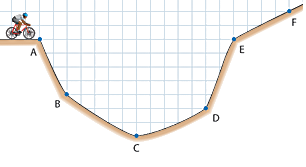
\includegraphics{Conservation_Kinetic_Potential}
    \end{center}
    Where would the bicyclist have the...
    \begin{enumerate}
        \item Highest potential energy?
        \item Lowest potential energy?
        \item Highest kinetic energy?
        \item Highest speed?
    \end{enumerate}
    Would the bicyclist's ..... be higher at A or C?
    \begin{enumerate}
        \item Kinetic energy
        \item Potential energy
        \item Total energy
    \end{enumerate}
    Suppose the bicyclist lets off the brakes and coasts down into the valley without pedaling. Even if there is no friction or air resistance to slow him down, what is the farthest point the bicyclist could reach without pedaling?
\end{exmp}
You can solve this problem by using some facts about energy.
\newline
First, use the fact that kinetic energy is energy in the form of motion, and that kinetic energy is proportional to the mass of what's moving and the square of the speed of the motion.
\begin{enumerate}
    \item That means the bicyclist has kinetic energy whenever he's moving, and that the faster he moves the more kinetic energy he has.
\end{enumerate}
Next, use the fact that potential energy is energy from the potential action of a force, and that potential energy is proportional to the strength of the force and to the distance over which it can act.
\begin{enumerate}
    \item In this case, the force is the force of gravity pulling the bicyclist down, and the distance over which it can act is his height above the bottom of the valley. (Once he reaches the bottom of the valley, gravity can't pull him any further down) That means the bicyclist's potential energy will be higher the higher he is above the valley floor.
\end{enumerate}
Finally, and most importantly, use the Principle of Conservation of Energy, which tells you that energy can neither be created nor destroyed. 
\begin{enumerate}
    \item That means as the bicyclist loses potential energy coasting downhill, he must gain an equal amount of kinetic energy (by speeding up), so that his total energy must stay constant.
    \item Similarly, when the bicyclist gains potential energy by coasting up the far side of the valley, he must lose kinetic eneryg (by slowing down), so that his total energy must stay constant.
\end{enumerate}
Now let's apply these general principles to the specific questions in this problem:
\begin{enumerate}
    \item Since his potential energy is proportional to his height above the bottom of the valley, the bicyclist would have the highest potential energy at F and the lowest at C.
    \item Since his kinetic energy increases as his potential energy decreases, the bicyclist would have the highest kinetic energy where his potential energy is the lowest, at C.
    \item Likewise, since kinetic energy is proportional to the square of speed, the speed of the bicyclist is the highest when the kinetic energy is the highest - at C. 
    \item At the entrance to the valley, the bicyclist isn't moving, so he has no kinetic energy. That means his total energy is equal to his potential energy. For the bicyclist to be able to coast up the other side of the valley to a point higher than the valley enterance (for example to point F), he'd have to have a potential energy higher than his total energy - which is impossible! \\
    Therefore, even if he loses no energy to friction with the road or air, the bicyclist can go no higher than the valley entrance without pedaling. That means the furthest point he can reach is E. 
    \item Since A is higher than C, the bicyclist's potential energy would be higher and his kinetic energy would be lower. The total energy, however, would be the same at both points.
\end{enumerate}

\section*{Calculating Solubility}
\begin{exmp}
    A geochemist in the field takes a 50mL sample of water from a rock pool lined with crystals of a certain mineral compound X. He notes the temperature of the pool, 17C, and caps the sample carefully. Back in the lab, the geochemist filters the sample and then evaporates all the water under vacuum. Crystals of X are left behind. The researcher washes, dries and weighs the crystals. They weigh 1.7g.
    \begin{enumerate}
        \item Using only the information above, can you calculate the solubility of X in water at 17C? If so, calculate it.
    \end{enumerate} 
\end{exmp}
You can solve this problem by using the fact that the solubility of a solute is equal to its concentration in a saturated solution, and a saturated solution is a solution in which \emph{no more of the solute will dissolve}.
\begin{enumerate}
    \item You \emph{know} a solution is saturated when it's in contact with extra solute that refuses to dissolve. 
    \item If there is no undissolved solute, the solution may or may not be saturated.
\end{enumerate}
In this case, you know that the solution must be saturated in X, since it's in contact with undissolved X. That means you \emph{can} calculate the solubility of X.
\newline
THe solubility of X equals the concentration of X in the saturated solution - the mass of dissolved X divided by the volume of the solution:
\begin{equation*}
    \begin{aligned}
        \frac{1.7g}{50.0mL} = 0.03400... g/mL
    \end{aligned}
\end{equation*}
There are 2 sig figs in 1.7g and 3 in 50.0 mL. So your calculated answer should have 2 sig figs.

\section*{Using the solubility of a compound to calculate $K_{sp}$}
\begin{exmp}
    The solubility of \ce{CaCO3} in water at 25C is measured to be 0.0067 g/L. Use this information to calculate $K_{sp}$ for \ce{CaCO3}.
\end{exmp}
In a saturated solution, the last bit of undissolved \ce{CaCO3} will be in equilibrium with the dissolved ions:
\begin{equation*}
    \begin{aligned}
        \ce{CaCO3(s) <=> Ca^2+(aq) + CO3^2-(aq)}
    \end{aligned}
\end{equation*}
That means the equilibrium molarities of the ions must be related to $K_{sp}$ through the $K_{sp}$ expression equation:
\begin{equation*}
    \begin{aligned}
        \ce{K_{sp} = [Ca^2+][CO3^2-]} \text{ CaCO3 doesn't appear here because it's present as a pure solid.}
    \end{aligned}
\end{equation*}
To use this equation, you first need to convert the equilibrium solubility of \ce{CaCO3} to the equilibrium molar solubility. Dividing grams per liter by the molar mass of \ce{CaCO3} will convert to moles per liter:
\begin{equation*}
    \begin{aligned}
        \frac{0.0067 g/L}{100.086 g/mol} = 6.694...*10^{-5}M
    \end{aligned}
\end{equation*}
Now use the stoichiometry in the chemical equation to find the molarities of \ce{Ca^2+} and \ce{CO3^2-}
\begin{equation*}
    \begin{aligned}
        \ce{[Ca^2+]} = 6.694*10^{-5}\\
        \ce{[CO3^2-]} = 6.694*10^{-5}
    \end{aligned}
\end{equation*}
Now you can calculate $K_{sp}$: 
\begin{equation*}
    \begin{aligned}
        K_{sp} &= (6.694*10^{-5})(6.694*10^{-5})\\
            &= 4.481*10^{-9} \\
            &= 4.5*10^{-9}
    \end{aligned}
\end{equation*}

\section*{Using $K_{sp}$ to calculate the solubility of a compound}
\begin{exmp}
    Calculate the solubility of \ce{CaF2} in water at 25C. 
\end{exmp}
In a saturated solution, the last bit of undissolved \ce{CaF2} will be in equilibrium with the dissolved ions:
\begin{equation*}
    \begin{aligned}
        \ce{CaF2 <=> CA^2+ + 2F-}
    \end{aligned}
\end{equation*}
That means you can calculate the equilibrium molarities of the ions from the $K_{sp}$ expression equation.
\begin{equation*}
    \begin{aligned}
        K_{sp} = \ce{[Ca^2+][F-]^2} \text{CaF2 doesn't appear here since its a pure solid.}
    \end{aligned}
\end{equation*}
As always when solving equilibrium composition problems, it's helpful to begin by setting up an ICE table. Let x stand for the moles per liter of \ce{CaF2} that dissolves:
\begin{center}
    \begin{tabular}{ c c c}
        X & $\ce{[Ca^2+]}$ & $\ce{[F^-]}$ \\
        I & 0 & 0  \\
        C & x & 2x \\
        E & x & 2x
    \end{tabular}
\end{center}
There's no column for \ce{CaF2}. Since it's present as the pure solid, it can't change concentration, and can't be in the reaction table.
\newline
Now substitute the expresion from the "equilibrium" line of the reaction table into the $K_{sp}$ expression:
\begin{equation*}
    \begin{aligned}
        K_{sp} &= x * (2x)^2 \\
        K_{sp} &= 4x^3 \text{Simplify.}\\
        x &= (K_{sp}/4)^{1/3} \text{Solve for x.} \\
         &= (K_{sp}/4)^{1/3} \text{Substitute Ksp from ALEKS data tab.} \\
         &= ((3.45*10^{-11})/4)^{1/3} \\
         &= 2.051*10^{-4} moles/Liter
    \end{aligned}
\end{equation*}
Multiply by molar mass to find grams per liter dissolved:
\begin{equation*}
    \begin{aligned}
        (2.051*10^{-4} \frac{mol}{L})*(78.075 \frac{g}{mol}) = 0.01601 \frac{g}{L}
    \end{aligned}
\end{equation*}
%-------------------------------------------------------------------------------
\section*{Scratch Work}

\begin{equation*}
    \begin{aligned}
        &0.521 = \frac{(4+2x)(x)}{(1.2-x)(2.4-x)} \\
        &0.521 * (1.2-x)(2.4-x) = 4x+ 2x^2 \\ 
        &K * (I_a - x)(I_b - x) = (I_c + 2x)(I_d + x)\\
        &K * (I_a* I_b - (I_a + I_b)x + x^2) = I_c* I_d - 2(I_c + I_d)x + 2x^2 \\
        &K(I_a* I_b) - K(I_a + I_b)x + Kx^2 = (I_c* I_d) - 2(I_c + I_d)x + 2x^2 \\
        &K(I_a* I_b) - (I_c* I_d) + K(I_a + I_b)x - 2(I_c + I_d)x + Kx^2 - 2x^2 = 0 \\
        &0.521(1.2*2.4) - (4*0) + 0.521(1.2 + 2.4)x - 2(4+0)x + 0.521x^2 - 2x^2 = 0 \\
        &1.50048 + 1.87560x - 8x - (0.521-8)x^2 = 0
    \end{aligned}
\end{equation*}

\begin{tabular}{c|c@{}c@{}c@{}c@{}c@{}c@{}c}
    \hline
    X   & $[HBrO]$ & ${}+{}$ & $[H_2O]$ & ${}\leftrightharpoons{}$ & $[BrO^-]$ & ${}+{}$ & $[H_3O^+]$ \\
    \hline
    I   &  0.88    &&     &&  0   && 0  \\
    C   &   -x   &&     &&  x   &&  x \\
    E   &   0.88-x   &&     &&   x  && x  \\      
\end{tabular}

\begin{equation*}
    \begin{aligned}
        K_a = \frac{x^2}{0.88-x} \\
        2.3*10^-9 * 0.88 = x^2 \\
        x = 4.49889*10^{-5} \\
        pH = -log_{10}(x)     
    \end{aligned}
\end{equation*}

For any weak acid with Ka and inital concentration M assuming small x approximation:
\begin{equation}
    pH = - log_{10}(K_a*M)
\end{equation}

\begin{tabular}{c|c@{}c@{}c@{}c@{}c@{}c@{}c}
    \hline
    X   & $[HA]$ & ${}+{}$ & $[H_2O]$ & ${}\leftrightharpoons{}$ & $[H_3O^+]$ & ${}+{}$ & $[A^-]$ \\
    \hline
    I   &  1.9    &&     &&  0   && 0  \\
    C   &   -x   &&     &&  x   &&  x \\
    E   &   1.9-x   &&     &&   x  && x  \\      
\end{tabular}

\begin{equation*}
    \begin{aligned}
        K_a &= \frac{[H_3O^+][A^-]}{[HA]} \\
        K_a &= \frac{x^2}{1.9-x} \\
        K_a &= \frac{x^2}{1.9} \\
        6.0*10^{-6}*(1.9) &= x^2 \\
        x &= \sqrt{6.0*10^{-6}*(1.9)} \\
        [H^+] &= 0.00337... \\
        pH &= -log_{10}\left(\sqrt{6.0*10^{-6}*(1.9)}\right) \\
        pH &= 2.47154757433
    \end{aligned}
\end{equation*}

If K = 5, then the ratio of products to reactants will be 5 - I'm assuming that we can ignore the number of atoms in each molecule so we can make it easier to determine whether the solution is in equilibrium.
\begin{equation*}
    \begin{aligned}
        \text{Product} = 8 \\
        \text{Reactant} = 2 \\
        \frac{P}{R} = \frac{8}{2} = 4 \\
    \end{aligned}
\end{equation*}
Thus the solution isn't in equilibrium.

...For K = 11
\begin{equation*}
    \begin{aligned}
        \text{Product} = 11 \\
        \text{Reactant} = 1 \\
        \frac{P}{R} = \frac{11}{1} = 11 \\
    \end{aligned}
\end{equation*}

Finding pOH - done by subtracting pH from 14:
\begin{equation*}
    \begin{aligned}
        pOH = 14 - pH
    \end{aligned}
\end{equation*} 

Finding \% evaporated since isolated:
\begin{enumerate}
    \item Parsons Concentration is 69 $\frac{g}{L}$
    \item Regular Concentration is 2.2 $\frac{g}{L}$
    \item Setting up equation:
    \begin{equation*}
        \begin{aligned}
            C_0 = C_i = 2.2 \frac{g}{L} \\
        \end{aligned}
    \end{equation*}
    \item Presently, 
    \begin{equation*}
        \begin{aligned}
            xC_0 = 69 \\
            C_0 = 2.2 \\
            x(2.2) = 69 \\
            x = \frac{69}{2.2}  = 31.36 \text{times more salty}\\
            \frac{100}{31.36} = 2.75\% 
            \text{Percent Evaporated} = 100 - 2.75 = 97.25
        \end{aligned}
    \end{equation*}
\end{enumerate}

Finding Equilibrium Constant for Reaction: \\
\ce{H2C2O4 -> 2H^+ + C2O4^2-}
K = \ce{\frac{[H]^2[C2O4]}{[H2C2O4]}}

\begin{equation*}
    \begin{aligned}
        \ce{2NH3_(g) <=> N2_(g) + 3H2_(g)}
    \end{aligned}
\end{equation*}

Finding inital concentration for ammonia:
\begin{equation*}
    \begin{aligned}
        &M = \frac{[NH_3]}{V} = \frac{2.2}{0.2} \\
        &M = 11M
    \end{aligned}
\end{equation*}

\begin{tabular}{c|c@{}c@{}c@{}c@{}c}
    \hline
    X   &   $[2NH_3]$ & ${}\leftrightharpoons{}$ & $[N_2]$ & ${}+{}$ & $[3H_2]$\\
    \hline
    I   & 11          &&   0                           &&  0       \\
    C   & -2x         &&   x                           &&  3x      \\
    E   & 11 - 2x     &&   x                           &&  3x      \\
    \hline
\end{tabular}

Creating $K_c$:
\begin{equation*}
    \begin{aligned}
        K_c &= \frac{[N_2][H_2]^3}{[NH_3]^2} \\
            &= \frac{[x][3x]^3}{[11-2x]^2} \\
    \end{aligned}
\end{equation*}

Plugging in $[H_2] = 1.7/0.2 = 8.5M$ and applying small-x approximation:
\begin{equation*}
    \begin{aligned}
        K_c &= \frac{[N_2][H_2]^3}{[NH_3]^2} \\
            &= \frac{[x][8.5]^3}{[11]^2} \\
    \end{aligned}
\end{equation*}

\begin{equation*}
    \begin{aligned}
        K = \ce{\frac{[H_2] [Cl_2]}{[HCl^2]}}
    \end{aligned}
\end{equation*}
Finding M/L for HCl:
\begin{equation*}
    \begin{aligned}
        M = \frac{0.39mol}{17L} = 2.3*10^{-2}M
    \end{aligned}
\end{equation*}

Important for finding K - since HCl is a strong acid, there will be no HCl at equilibrium ideally. And since we have 2M HCl for H2 and Cl2 respectively, the final K will be $\left(2.3*10^-2\right)^2$

\begin{tabular}{c|c@{}c@{}c@{}c@{}c}
    \hline
    X   &   $[2HCl]$ & ${}\leftrightharpoons{}$ & $[H_2]$ & ${}+{}$ & $[Cl_2]$\\
    \hline
    I   &  0.023     &&   0                            &&  0       \\
    C   &       -2x      &&   x                           &&  x      \\
    E   &   0.023 - 2x     &&   x                           &&  x      \\
    \hline
\end{tabular}

\begin{equation*}
    \begin{aligned}
        K &= \ce{\frac{[H_2] [Cl_2]}{[HCl^2]}} \\
        K &= \frac{x*x}{0.023 - 2x} \\
        (0.023 - 2x)K &= x^2 \\
        0.023K - 
    \end{aligned}
\end{equation*}



Ammonia decomposition:
\begin{equation*}
    \begin{aligned}
        \ce{2NH3 -> 3H2 + N2}
    \end{aligned}
\end{equation*}
if we have 4.5 atm of ammonia gas, and have 1.4 atm of nitrogen gas in a 5L 

Create ICE Table \\
\begin{tabular}{c|c@{}c@{}c@{}c@{}c}
    \hline
    X   &   $[2NH_3]$ & ${}\leftrightharpoons{}$ & $[N_2]$ & ${}+{}$ & $[3H_2]$\\
    \hline
    I   &       4.5     &&   0                            &&  0       \\
    C   &       -2x      &&   x                           &&  3x      \\
    E   &   4.5 - 2x     &&   x                           &&  3x      \\
    \hline
\end{tabular}
\begin{equation*}
    \begin{aligned}
        K_P &= \frac{[N_2] [H_2]^3}{[NH_3]^2} \\
            &= \frac{x(3x)}{(4.5-2x)^3} \\
            &= \frac{1.4(3*1.4)}{(4.5-2*1.4)^3} 
    \end{aligned}
\end{equation*}

Sulfur dioxide and oxygen gas react too make sulfur trioxide reaction:
\begin{equation*}
    \begin{aligned}
        \ce{2SO2 + O2 -> 2SO3}
    \end{aligned}
\end{equation*}

Create ICE Table \\
\begin{tabular}{c|c@{}c@{}c@{}c@{}c}
    \hline
    X   &   $[2SO_2]$ & ${}+{}$ & $[O_2]$ & ${}\leftrightharpoons{}$ & $[2SO_3]$ \\
    \hline
    I   &       0.3066       &&   0.4133        &&  0       \\
    C   &       -2x      &&   -x        &&  2x      \\
    E   &       0.3066 - 2x     &&   0.4133 - x        &&  2x      \\
    \hline
\end{tabular}

\begin{equation*}
    \begin{aligned}
        K_b = \ce{\frac{[(CH3)2NH^+][OH-]}{(CH3)2NH}}
    \end{aligned}
\end{equation*}

\begin{equation*}
    \begin{aligned}
        K_b = \ce{\frac{[(CH3)3NH+][OH-]}{(CH3)3N}}
    \end{aligned}
\end{equation*}

Original
\begin{equation*}
    \begin{aligned}
        O = 4 \\
        d = 6 
    \end{aligned}
\end{equation*}
Box C
\begin{equation*}
    \begin{aligned}
        O = 4 \\
        d = 6 
    \end{aligned}
\end{equation*}

Box E
\begin{equation*}
    \begin{aligned}
        O = 5 \\
        d = 5 
    \end{aligned}
\end{equation*}

\subsection*{CHEM Lab Exp. 3 - Buffers}
\subsubsection*{Introduction} 
To prepare, determine, and compare the buffering capacity of various solutions.
\subsubsection*{Method}
Part A - Solution Prep:
\begin{enumerate}
    \item Clean glassware with soap and brushes in lab. Rinse and dry beakers, shaking excess water from clean test tubes.
    \item Label test tubes 1-6.
\end{enumerate}

\end{document}